%%%%%%%%%%%%%%%%%%%%%%%%%%%%%%%%%%%%%%%%
%%     Title and ToC
%%%%%%%%%%%%%%%%%%%%%%%%%%%%%%%%%%%%%%%%
% titlepage
\frame{
  \maketitle
}

\setcounter{footnote}{0}
\begin{frame}[noframenumbering]
\frametitle{The pbdR Core Team}
\begin{minipage}{3.6cm}
Wei-Chen Chen$^1$ \\
George Ostrouchov$^{1,2}$ \\
Pragneshkumar Patel$^2$ \\
Drew Schmidt$^2$ \\[2ex]
\end{minipage}
\begin{minipage}{7cm}
  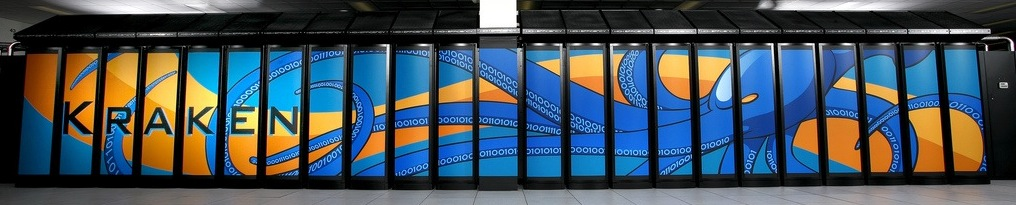
\includegraphics[width=7cm]{../common/pics/kraken1wide} \\
  \tiny\bf 112,896 Cores in 18,816 Nodes with 147 TB Memory \\
\end{minipage}

\vspace{-1.5em}
\begin{block}{Support}\tiny
  This work used resources of the \textcolor{blue}{Oak Ridge
    Leadership Computing Facility} at the Oak Ridge National
  Laboratory, which is supported by the Office of Science of the
  U.S. Department of Energy under Contract No. DE-AC05-00OR22725. This
  work also used resources of \textcolor{blue}{National Institute for
    Computational Sciences} at the University of Tennessee, Knoxville,
  which is supported by the Office of Cyberinfrastructure of the
  U.S. National Science Foundation under Award
  No. ARRA-NSF-OCI-0906324 for NICS-RDAV center. This work used
  resources of the Newton HPC Program at the University of Tennessee,
  Knoxville.

  \tiny \vspace{1em}$^1$Oak Ridge National Laboratory. Supported in
  part by the project ``Visual Data Exploration and Analysis of
  Ultra-large Climate Data'' funded by U.S. DOE Office of Science
  under Contract No. DE-AC05-00OR22725.

  \vspace{1em}$^2$University of Tennessee. Supported in part by the
  project ``NICS Remote Data Analysis and Visualization Center''
  funded by the Office of Cyberinfrastructure of the U.S. National
  Science Foundation under Award No. ARRA-NSF-OCI-0906324 for
  NICS-RDAV center.
\end{block}
\end{frame}

\begin{frame}
\frametitle{About This Presentation}
 \begin{block}{Downloads}
  This presentation and supplemental materials are available at:
  \begin{center}
  \url{http://r-pbd.org/tutorial}
  \end{center}
  Sample R scripts and pbs job scripts available on Nautilus from:\\
  \centering\code{/lustre/medusa/proj/pbdR/tutorial/scripts.tar.gz}
 \end{block}
\end{frame}


\begin{frame}
\frametitle{About This Presentation}
 \begin{block}{\emph{Speaking Serial R with a Parallel Accent}}
  The content of this presentation is based in part on the \pkg{pbdDEMO} 
vignette \emph{Speaking Serial R with a Parallel Accent}\\[.4cm]
  \url{http://goo.gl/HZkRt}\\[.4cm]
  It contains more examples, and sometimes added detail.
 \end{block}
\end{frame}


\begin{frame}
\frametitle{About This Presentation}
 \begin{block}{Installation Instructions}
  Installation instructions for setting up a pbdR environment are available:
  \begin{center}
  \url{http://r-pbd.org/install.html}
  \end{center}
  This includes instructions for installing R, MPI, and pbdR.
 \end{block}
\end{frame}



% \begin{frame}%[allowframebreaks=0.8]
% \frametitle{About This Presentation}
%  \begin{block}{Conventions}
%   \begin{itemize}
%     \item We use ``{\Huge$ .$}'' as a decimal mark, not ``{\Huge$,$}''.  E.g., ``one thousand and one half'' is written ``$1,000.5$'', not ``$1.000,5$''.
%     \item We will use special suffixes to denote distributed objects (ones not stored entirely on a single processor).\\
%     \code{.spmd} denotes a distributed object, while\\
%     \code{.dmat} denotes a distributed object which is of class \code{ddmatrix}\\
%     No suffix means the object is global (common to all processors)\\[.2cm]
%     Neither of these suffices carries semantic meaning.
%     \end{itemize}
%  \end{block}
% \end{frame}



\begin{frame}[fragile]
\frametitle{About This Presentation}
 \begin{block}{Conventions For Code Presentation}
We will use two different forms of syntax highlighting.  One for displaying results from an interactive R session:
\begin{lstlisting}[backgroundcolor=\color{white},basicstyle=\ttfamily\color{dkgray}\scriptsize,keywordstyle=\color{black}, 
  commentstyle=\color{orange},stringstyle=\color{mauve}]
R> "interactive"
[1] "interactive"
\end{lstlisting}
and one for presenting R scripts
\begin{lstlisting}
"not interactive"
\end{lstlisting}
 \end{block}
\end{frame}



\begin{frame}[noframenumbering,shrink]
\frametitle{Contents}
\small
\tableofcontents[hideallsubsections]
\end{frame}

\setcounter{framenumber}{0}
